\chapter{成像和行为} \label{chap:chap6}

为了用生物学术语解释生物体的行为,有必要协调生物学过程的测量(例如,动作电位、血流、神经递质的释放)与认知和运动输出的测量。
然而,将生物学和行为学的测量方法联系起来是具有挑战性的
对非人类动物进行精确的神经测量和侵入性技术是可能的,但其中许多物种的行为库相对有限。
此外,直接测量或侵入性地操纵健康人类的神经活动要困难得多,健康人类是具有最先进和最多样化行为的物种。
因此,现代神经科学的核心努力一直是开发新方法,以从人脑中获取精确的生物学测量值,并在非人类动物中模拟人类行为。


人类测量生物过程并将其与行为联系起来的主要方法是\textit{功能性核磁共振成像}。
\textit{脑电图}、\textit{正电子发射断层扫描}和\textit{近红外光谱}等其他测量人脑功能的成像方法各有长处。
然而,由于多种原因,功能性核磁共振成像特别适合研究人类行为的神经基础。
首先,它是非侵入性的:它不需要手术、电离辐射或其他破坏性干预。
其次,它可以在短时间内(以秒为单位)测量大脑功能,这使其能够捕捉心理过程和行为的动态方面。
第三,它同时测量整个大脑的活动,为研究多个大脑区域如何相互作用以调节复杂行为的提供了机会。
因此,本章的重点是功能性核磁共振成像。


我们首先解释功能性核磁共振成像实验如何工作的技术细节以及通常如何收集数据。 
然后我们解释如何分析功能性核磁共振成像数据以及它们如何提供对人类行为和思想的洞察力。 
然后,我们将使用来自感知、记忆和决策领域的示例,对从功能性核磁共振成像中学到的内容进行更概念性的概述。
最后,我们考虑功能性核磁共振成像的优势和局限性,并讨论它可以支持的关于大脑和行为的推断类型。


虽然本章的重点是健康大脑的成像和行为,但功能性核磁共振成像也有可能改变我们诊断和治疗精神和神经疾病的方式。
几乎所有此类疾病(例如,孤独症、精神分裂症、抑郁症、\textit{进食障碍})除了特定大脑区域和细胞类型的破坏之外,还涉及大规模回路动力学的变化。
对健康大脑回路如何调节心理过程和行为的基础研究,结合在临床人群中测量这些相同回路活动的能力,为理解疾病和功能失调行为带来了巨大希望。



\section{功能性核磁共振成像实验测量神经血管活动}

功能性核磁共振成像实验使研究人员能够根据响应神经活动而发生的局部血氧水平变化来追踪大脑功能。
与所有形式的核磁共振成像一样,功能性核磁共振成像需要高度专业化的设备和复杂的计算机程序。
在本节中,我们首先考虑如何使用核磁共振成像对大脑\textit{结构}成像的基本原理,然后解释功能性核磁共振成像如何将此功能扩展到对大脑\textit{活动}成像。


每台核磁共振成像机器的核心都是强大的磁铁。
磁场强度以\textit{特斯拉}为单位进行量化,大多数现代\textit{核磁共振成像}机器都是 3 \textit{特斯拉}。
使用像 7 \textit{特斯拉}这样更高的场强会提供了一些优势,包括对皮层进行更高分辨率成像的可能性。
此类机器还没有普及,层特定成像还处于起步阶段,所以我们关注 3 \textit{特斯拉}机器的能力和配置。


% % The outside of an MRI machine looks like a tunnel, known as the “bore” of the magnet. 
核磁共振成像仪的外部看起来像一条隧道,被称为磁铁的“孔”。
% Subjects lie on a bed with their head in a helmet-like head coil, which receives signals from the brain. 
受试者躺在床上,头戴头盔状的头部线圈,接收来自大脑的信号。
% Visual stimuli are typically viewed through a mirror on the head coil angled toward a screen at the back of the bore.
视觉刺激通常通过头部线圈上的镜子观察,镜子与孔后部的屏幕成一定角度。
% Auditory stimuli are presented through headphones. 
听觉刺激通过耳机呈现。
% Behavior is typically measured in terms of manual responses with a button box and/or eye movements with an eye tracker.
行为通常根据使用按钮框的手动响应和/或使用眼动仪的眼球运动来衡量。
% This apparatus constrains which experimental tasks are possible. 
该设备限制了哪些实验任务是可能的。
% However, fMRI is flexible in other ways, including that it can be performed and repeated without harm in many different types of subjects, from children to the elderly, whether healthy or suffering from a disorder.
然而,功能性核磁共振成像在其他方面也很灵活,包括它可以在许多不同类型的受试者身上进行和重复,而不会造成伤害,从儿童到老人,无论是健康的还是患有疾病的。


% What does fMRI measure? 
功能性核磁共振成像测量什么?
% There are two fundamental concepts that we will discuss in turn, first magnetic resonance and then neurovascular coupling (Figure 6–1).
我们将依次讨论两个基本概念,首先是\textit{磁共振},然后是\textit{神经血管耦合}(图~\ref{fig:6_1})。


\begin{figure}[htbp]
	\centering
	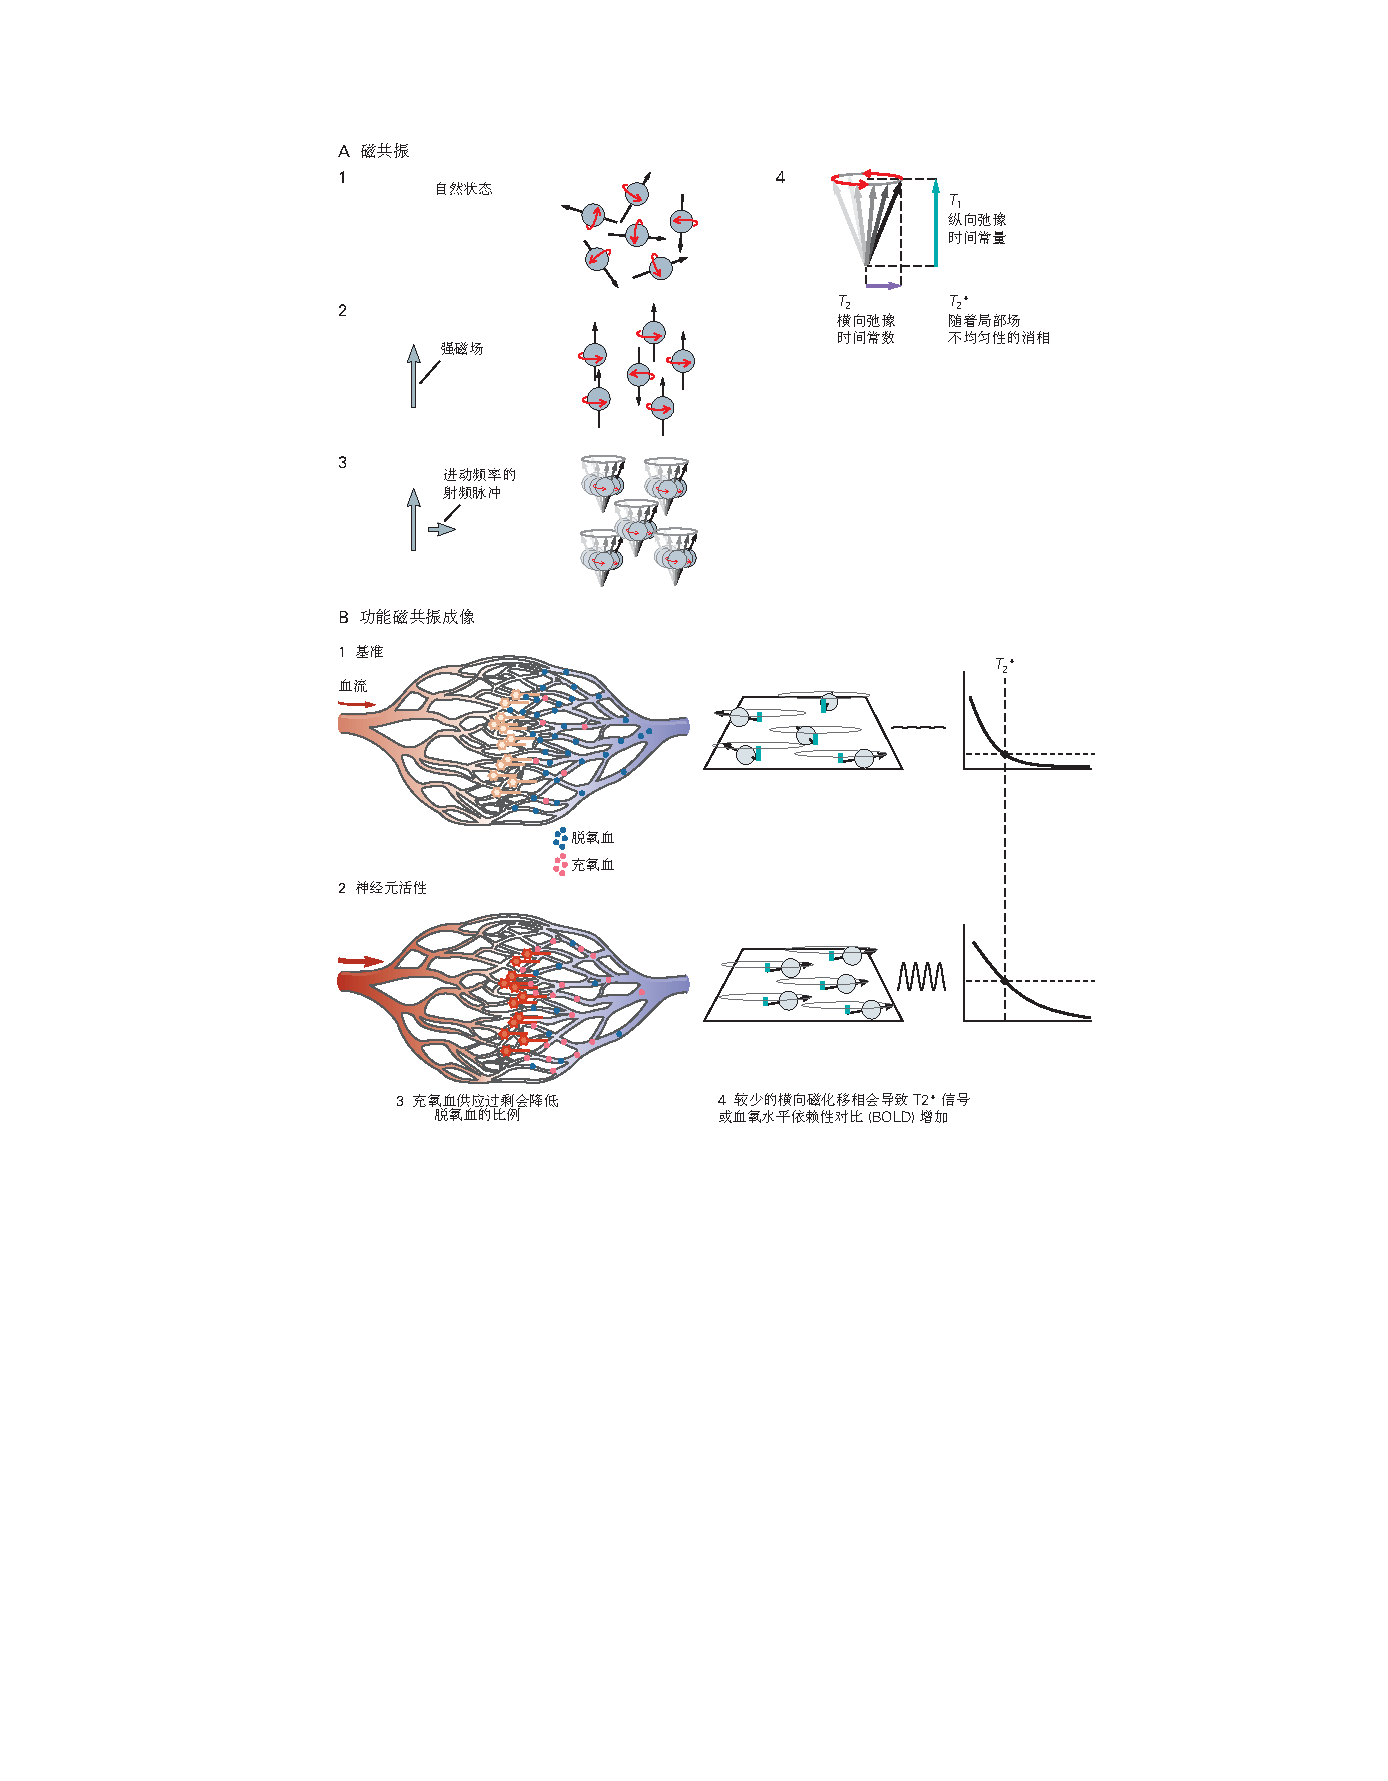
\includegraphics[width=0.9\linewidth]{chap06/fig_6_1}
	\caption{\textit{功能性核磁共振成像}如何测量神经活动。
		\textbf{A.} 在核磁共振环境之外,大脑中氢原子中的质子围绕指向随机方向的轴旋转(1)。
		当大脑进入核磁共振成像孔的强磁场时,这些轴的子集与该磁场对齐,这被称为纵向磁化(2)。
		这些质子可以通过发射射频脉冲来测量,射频脉冲会感应出垂直于强磁场的较弱磁场。
		这会使质子与强场错位,强场现在充当扭矩,导致质子自旋轴在横向平面上以弧形进动。
		选择射频脉冲的频率以与质子的进动速率共振,而质子的进动速率又取决于磁场强度(3)。
		当射频脉冲停止时,质子最初继续同步进动,在头部周围的接收线圈中感应出相同频率的交流电。
		这些信号可用于通过应用磁梯度来生成图像,磁梯度可调整整个大脑正交方向的场强。
		这会在大脑的不同点产生不同的共振频率,从而可以识别接收信号的来源。
		横向磁化随时间消散,信号丢失。
		这种弛豫发生在质子释放热力学能量并且它们的轴返回纵向方向(T1)时,并且由于质子在横向平面中由于与其他原子和分子的局部相互作用而变得不同步(T2),并且由于质子中的不均匀性 磁场(T2 *)(4)。
		\textbf{B.} 由于血液的磁性,磁共振可用于估计功能性核磁共振成像中的神经元活动。
		% 活跃时需要更多的血
		当大脑区域处于基线状态时,脱氧血与充氧血的比例高于该区域活跃时的比例。
		% 脱氧血红蛋白(即没有携带氧的血红蛋白)中的每个铁原子都有4个未配对的电子,使得脱氧血红蛋白具有微弱的顺磁性;
		% 但氧合血红蛋白(即携带了氧气的血红蛋白)中的铁原子没有未配对电子,使得氧合血红蛋白具有抗磁性。
		脱氧血与磁场相互作用,导致局部不均匀性,从而扭曲进动速率并破坏横向平面中质子的同步,导致更快的 T2 * 衰减和更低的\textit{血氧水平依赖}信号(1)。
		神经元活动导致代谢需求(2),进而导致输送过量的氧合血(3)。
		含氧血液不与磁场相互作用,因此活跃大脑区域的含氧量增加会减少场的不均匀性。
		反过来,这减少了质子在横向平面进动的相位差,导致更慢的 T2 * 衰减和更高的\textit{血氧水平依赖}信号(4)。}
	\label{fig:6_1}
\end{figure}



% fMRI Depends on the Physics of Magnetic Resonance
\subsection{功能性核磁共振成像取决于磁共振物理学}

% In general, MRI exploits the magnetic properties of hydrogen atoms, the dominant source of protons in the body, specifically the way each atom’s proton interacts with a strong magnetic field. 
一般来说,核磁共振成像利用氢原子的磁性,氢原子是体内质子的主要来源,特别是每个原子的质子与强磁场相互作用的方式。
% A key property of protons is that they intrinsically rotate around an axis. 
质子的一个关键特性是它们本质上围绕一个轴旋转。
% This spin gives protons angular momentum and a magnetic dipole along the axis, their own north and south poles. 
这种自旋给质子提供了角动量和沿它们自己南北极轴的\textit{磁偶极子}。
% Under normal circumstances, the directions of these dipoles are random for different protons.
在正常情况下,这些偶极子的方向对于不同的质子是随机的。
% When placed in a strong external magnetic field, however, a subset of the protons (how many is proportional to the field strength) align with the direction of this field, which extends from foot to head when lying in an MRI bore.
然而,当置于强外部磁场中时,质子的子集(数量与场强成正比)与磁场方向对齐,当位于核磁共振成像孔中时,质子从脚延伸到头部。


% In the case of a 3T magnet and hydrogen atoms, this speed is in the radiofrequency (RF) range.

% An important step toward measuring a signal from protons is to push them out of alignment with this main field. 
测量质子信号的一个重要步骤是将它们推离这个主场。
% To understand why, it is helpful to think about a familiar object, the gyroscope. 
要理解其中的原因,不妨想想一个熟悉的物体,即陀螺仪。
% If a still gyroscope is tipped out of vertical balance, it will just fall over. 
如果一个静止的陀螺仪失去垂直平衡,它就会翻倒。
% However, if you spin the gyroscope before tipping it, inertial forces will prevent it from falling over. 
但是,如果在倾斜陀螺仪之前先旋转它,惯性力会防止它翻倒。
% The axis around which the gyroscope is spinning will itself begin to rotate around the vertical axis. 
围绕自身轴旋转的陀螺仪将开始围绕垂直轴旋转。
% This precession occurs because gravity exerts a vertical torque on the tilted gyroscope, pulling its center of mass down so that it pivots around its bottom point and traces out a circle in the transverse plane (looking from above).
发生这种进动是因为重力对倾斜的陀螺仪施加垂直扭矩,将其质心拉下,使其围绕其底部点旋转并在横向平面(从上方看)中划出一个圆圈。 
% Something similar happens to a proton that is tilted with respect to the strong magnetic field: The field applies a torque and the orientation of the rotational axis precesses around the field direction. 
相对于强磁场倾斜的质子也会发生类似的情况:磁场施加扭矩,旋转轴的方向围绕磁场方向进动。
% The speed of precession, or the resonant frequency, is determined by the Larmor equation, according to the field strength and a gyromagnetic ratio specific to each type of atom. 
进动速度或共振频率由\textit{拉莫尔方程}根据场强和每种原子特有的旋磁比确定。 
对于 3 \textit{特斯拉}磁体和氢原子,该速度处于\textit{射频}范围内。



% But how do protons get tipped out of alignment in the first place to enable precession?
但是,质子是如何从一开始就偏离排列以实现进动的呢? 
% The answer depends upon the same principle of torque. 
答案取决于扭矩的相同原理。 
% A second, weaker magnetic field is applied in a perpendicular direction (eg, front to back of the head), introducing another torque that pulls protons away from alignment with the strong field. 
第二个较弱的磁场在垂直方向(例如,从头部的前部到后部)施加,引入另一个扭矩,将质子拉离与强磁场对齐的位置。
% This misalignment causes precession about the direction of the strong field by allowing the strong field to act as a torque. 
这种未对准通过允许强场充当扭矩而导致围绕强场的方向的进动。
% Complicating matters, this precession makes protons a moving target for the weaker magnetic field that is needed to cause misalignment in the first place. 
使事情复杂化的是,这种进动使质子成为首先导致错位所需的较弱磁场的移动目标。
% This is solved by generating the second field using a transmit coil in the MRI machine, through which alternating current is passed to deliver an RF pulse at the resonant frequency of the protons. 
这是通过使用核磁共振仪中的发射线圈生成第二个场来解决的,交流电通过该线圈以在质子的共振频率下传递射频脉冲。
% This induces a perpendicular magnetic field that rotates in lockstep with the precession. 
这会产生一个垂直磁场,该磁场会随着进动同步旋转。
% This RF pulse is sustained as long as needed to generate a specified change in the spin orientation of protons away from the strong field direction (eg, 90°). 
该射频脉冲的持续时间与产生质子自旋方向远离强场方向(例如 90°)的指定变化所需的时间一样长。
% This change is known as the flip angle and is often chosen to maximize signal according to the Ernst equation.
这种变化被称为翻转角,通常根据 \textit{能斯特方程}选择它来最大化信号。


% Once the desired flip angle has been achieved, the RF pulse is stopped in order to measure the composition of tissue. 
一旦达到所需的翻转角,射频脉冲就会停止以测量组织的成分。
% At this point, protons are precessing around the strong magnetic field and tilted heavily into the transverse plane. 
此时,质子在强磁场周围进动并严重倾斜到横向平面中。
% This is akin to a bar magnet spinning on a table, where the north and south poles take turns passing any given location. 
这类似于在桌子上旋转的条形磁铁,北极和南极轮流经过任何给定位置。
% If a coil is placed nearby, the spinning magnet induces a current in the wire that reverses as the poles alternate. 
如果在附近放置一个线圈,旋转的磁铁会在电线中感应出电流,该电流会随着磁极交替而反转。
% This is what the receiver head coil in an MRI machine measures: alternating current induced by protons precessing synchronously (note: this is the same principle as described earlier for how the transmit coil works, just reversed). 
这就是核磁共振成像仪中的接收头线圈所测量的:由同步进动的质子感应的交流电(注意:这与前面描述的发射线圈的工作原理相同,只是相反)。
% The amount of current indicates the concentration of precessing protons.
电流量表示进动质子的浓度。


% Critically, the frequency of these measured signals reflects the speed of precession, which in turn depends on the strength of the magnetic field experienced by the tissue. 
至关重要的是,这些测量信号的频率反映了进动的速度,而进动的速度又取决于组织所经历的磁场强度。
% This can be used to generate three-dimensional images by imposing different gradients on the magnetic field (think of a staircase from higher to lower strength) that cause the Larmor frequency to vary systematically over space in the brain. 
这可用于通过在磁场上施加不同的梯度(想象从强度从高到低的阶梯)来生成三维图像,从而导致拉莫尔频率在大脑空间内系统地变化。
% During fMRI, one gradient is applied in a specific direction to select a slice of brain tissue. 
在功能性核磁共振成像期间,在特定方向上应用一个梯度以选择脑组织切片。
% The RF pulse can be tailored to the resonant frequency for the exact field strength at this gradient step, such that only protons in this slice are excited. 
可以针对此梯度步骤中的精确场强将射频脉冲调整为共振频率,以便仅激发该切片中的质子。
% The same logic is used with additional gradients in orthogonal directions to impose a two-dimensional matrix on the selected slice, with each unit volume in the matrix or voxel having a unique frequency and phase. 
相同的逻辑与正交方向上的附加梯度一起使用,以在所选切片上施加二维矩阵,矩阵或体素中的每个单位体积具有唯一的频率和相位。
% The head coil receives a composite signal with a mixture of these frequencies, but the signal can be decomposed to identify protons at every voxel in the slice.
头部线圈接收混合了这些频率的复合信号,但信号可以被分解以识别切片中每个体素处的质子。


进动质子还有另一个有助于核磁共振成像的重要特性:
在射频脉冲之后,头部线圈中感应的交流电开始衰减。
腐烂有不同的来源。
一个来源是进动质子向周围组织释放热力学能量(热量),就像陀螺仪最终会因摩擦而失去能量并翻倒。
当这种情况发生时,质子的自旋方向逐渐放松回到强磁场的方向,导致它们在横向平面内的进动减少,从而产生较少的信号。
这称为纵向弛豫并以时间常数 T1 发生。
第二种类型的衰变发生在质子仍在横向平面内进动时。
单个质子被其他原子的可变邻域包围,这些原子带有自己的弱磁场。
这会微妙地改变质子所经历的场强,导致其拉莫尔频率发生不可预测的变化。
而在\textit{射频}脉冲质子同步进动之后,这些局部相互作用会导致一些质子进动得更快或更慢。
由于它们越来越不同步,感应电流交替的可靠性降低,信号丢失。
这称为横向弛豫并以时间常数 T2 发生。 
质子的这种去相位也可能是强磁场本身的不均匀性造成的,包括它如何被置于磁场中的组织扭曲。 
来自局部相互作用和场失真的信号衰减具有时间常数 T2 *(发音为“T2-星”)。


这些不同的衰变源很重要,因为 T1 和 T2 时间常数因组织类型而异。 
因此,\textit{核磁共振成像}可以利用信号衰减来识别灰质、白质、脂肪和/或脑脊液。 
根据\textit{核磁共振成像}机器上设置的\textit{射频}脉冲、梯度和其他参数(统称为脉冲序列)的配置和时间,从不同体素接收的信号可以突出具有不同 T1 值的组织之间的对比度(T1 加权图像 ) 和/或不同的 T2 值(T2 加权图像)。 
例如,在 T1 加权图像中,白质比灰质更亮,而 T2 加权图像则相反。


测量脑功能的标准脉冲序列是\textit{平面回波成像}序列。 
\textit{平面回波成像}对\textit{功能性磁共振成像}有两个理想的特性:它非常快,允许在不到 100 毫秒的时间内从一个\textit{射频}脉冲获取整个切片,并且它对 T2 * 敏感,我们稍后将看到,这就是\textit{核磁共振成像}测量的方式 神经活动。 
在设计\textit{功能性磁共振成像}研究时,需要选择\textit{平面回波成像}序列的几个参数,包括在脑体积中获取多少切片(通常为 30-90); 
每卷多少时间(重复时间,通常为 1-2 秒); 使用何种体素分辨率(每个维度通常为 2-3 毫米); 
以及是否使用并行采集(例如,一次采集切片的多个部分和/或多个切片)。
这些选择是相互依存的,需要在速度、精度和信噪比之间进行权衡。



\subsection{功能性核磁共振成像依赖于神经血管耦合的生物学}

我们已经描述了磁共振的一般原理,但是故事的第二部分,神经血管耦合呢?
活跃的神经元消耗从血液中的氧气中获得的能量。 
因此,当大脑区域活跃时,血液中的氧合作用会在那一刻下降。
为了补充这些代谢资源,在接下来的几秒钟内流向局部的血液会增加。
供应超过需求,因此,与直觉相反,活跃的大脑区域中含氧(相对于脱氧)血液的比例更高。


要将此与磁共振联系起来,请记住 T2 * 衰变反映了由场不均匀性引起的质子相移。 
血液具有不同的磁性,具体取决于氧合作用:脱氧血液与磁场相互作用,因为血红蛋白中的铁是未结合的,而铁与氧结合的含氧血液则不会。
因此,脱氧血液会导致更快的 T2 * 衰减,并降低相对于含氧血液的信号。
这种信号差异称为血氧水平依赖性对比度。 
综上所述,用\textit{平面回波成像}序列测量的体素信号增加表明最近的神经元活动,因为伴随这种活动的局部血液氧合相对增加。
这种血氧水平依赖反应的时间曲线,称为血液动力学反应函数,看起来像一条长尾巴的钟形曲线,在局部神经活动后约 4 到 5 秒达到峰值,并在 12 到 15 秒后返回基线。
关于功能性核磁共振成像的物理学和生物学还有更多细节。 
此外,我们对这一切如何运作的理解仍在不断发展。 
例如,目前尚不清楚血氧水平依赖是否与单个神经元的放电或神经群体的活动更密切相关。 
同样,可能难以区分血液氧合作用增加是由局部兴奋或抑制增加引起的。 
更一般地说,神经血管耦合的机制(大脑如何知道何时何地输送含氧血液)仍然是个谜,人们越来越关注星形胶质细胞的功能作用。 
通过测量神经元活动精确部位的初始耗氧量(“初始下降”),也有可能获得更好的时间和空间分辨率,反映在脱氧血液中立即和局部上升,而不是延迟和更多弥漫性供氧过剩的血液。 
然而,即使理解不完全,功能性核磁共振成像也可以作为一种工具来定位由心理操作引起的人脑神经活动的变化。



\section{可以通过多种方式分析功能性核磁共振成像数据}

在进行功能性核磁共振成像实验时,研究人员将前面描述的神经血管测量与编程到人类受试者执行的计算机脚本中的认知任务联系起来。
该脚本通常会生成一系列运行,这些运行对应于连续的数据收集周期(即,连续的几个功能性核磁共振成像体积),通常持续 5 到 10 分钟。 
在每次运行中,通常通过显示视觉刺激或播放听觉刺激来向受试者展示几个试验。 
根据任务的不同,受试者可能会,例如,被动地查看或聆听刺激,对其做出决定,或将其存储在记忆中。 
按钮按下或眼球运动反应通常被收集为该试验中认知处理的行为指标。 
这些试验通常来自两个或多个任务条件,这些条件决定了刺激类型、任务难度或其他实验参数。 
在基本的减法设计中,试验分为实验条件和控制条件,它们是相同的,但有一个关键差异,其神经基础正在研究中。 
试验通常持续 2 到 10 秒,通常由几秒的可变或“抖动”间隔分隔。 
总之,此类会议通常持续长达 2 小时。


每个功能性核磁共振成像会话都会产生大量原始数据,在大脑中数十万个位置对血氧水平依赖响应进行数千次采样。 
这些数据如何转化为关于认知和行为的见解? 
许多功能性核磁共振成像分析方法都是可能的(方框~\ref{box:6_1}),但在大多数情况下,它们分为三类(图~\ref{fig:6_2})。 
我们首先描述所有三种类型共有的预处理步骤,然后解释每个步骤是如何进行的以及它能告诉我们什么。


\begin{proposition}[神经解剖学导航术语] \label{box:6_1}
	
	\quad \quad 与许多科学领域相比,大脑成像的基本方法具有显著的标准化。
	造成这种情况的一个主要原因是,自20世纪90年代中期\textit{功能性核磁共振成像}问世以来,广泛采用的软件包就已经问世。
	这些软件包是由研究小组创建和发布的,在流行之前,大多数都是开源的。
	
	\quad \quad 起初,它们包括用于预处理、对齐、分析模型和统计校正的工具。
	此后,他们引入了研究人员开发的新工具,包括非线性对齐、场图校正、非参数统计和并行化。
	
	\quad \quad 因此,几乎所有的\textit{功能性核磁共振成像}研究人员都使用一个或多个这样的包,至少在他们的分析管道中是这样。
	用于\textit{功能性核磁共振成像}分析的流行免费软件包包括:\href{https://afni.nimh.nih.gov}{AFNI}、\href{https://fsl.fmrib.ox.ac.uk}{FSL}、\href{https://www.fil.ion.ucl.ac.uk/spm}{SPM}。
	
	\quad \quad 除了这些专门的软件包,功能磁共振成像越来越多地被从数据科学的更普遍的角度来看待。
	这有两个原因。
	首先,功能磁共振成像产生了大量的数据,既包括在每次治疗中,也包括在已经进行的数千项研究中汇总的数据。
	因此,理解功能磁共振成像数据可以被认为是一个大数据问题。
	其次,数据非常复杂和嘈杂,感兴趣的认知信号很弱,很难找到。
	这带来了一个数据挖掘挑战,激励了许多计算机科学家。
	
	\quad \quad 这一趋势最具体的表现是\textit{功能性核磁共振成像}分析中机器学习的兴起。
	与数据科学的其他接触点包括与流数据的实时分析相关的挑战、网络分析和图论方法的应用、高性能计算集群和云系统的使用,以及研究人员公开共享数据的日益增长的实践(例如,\href{https://openneuro.org}{openneuro})、代码(在\href{https://github.com/}{GitHub}等服务上)和教育材料(例如,\href{https://brainiak.org/tutorials}{BrainIAK})。
	因此,脑成像领域将继续受益于计算机科学、工程、应用数学和统计学的进步。
	
\end{proposition}


\begin{figure}[htbp]
	\centering
	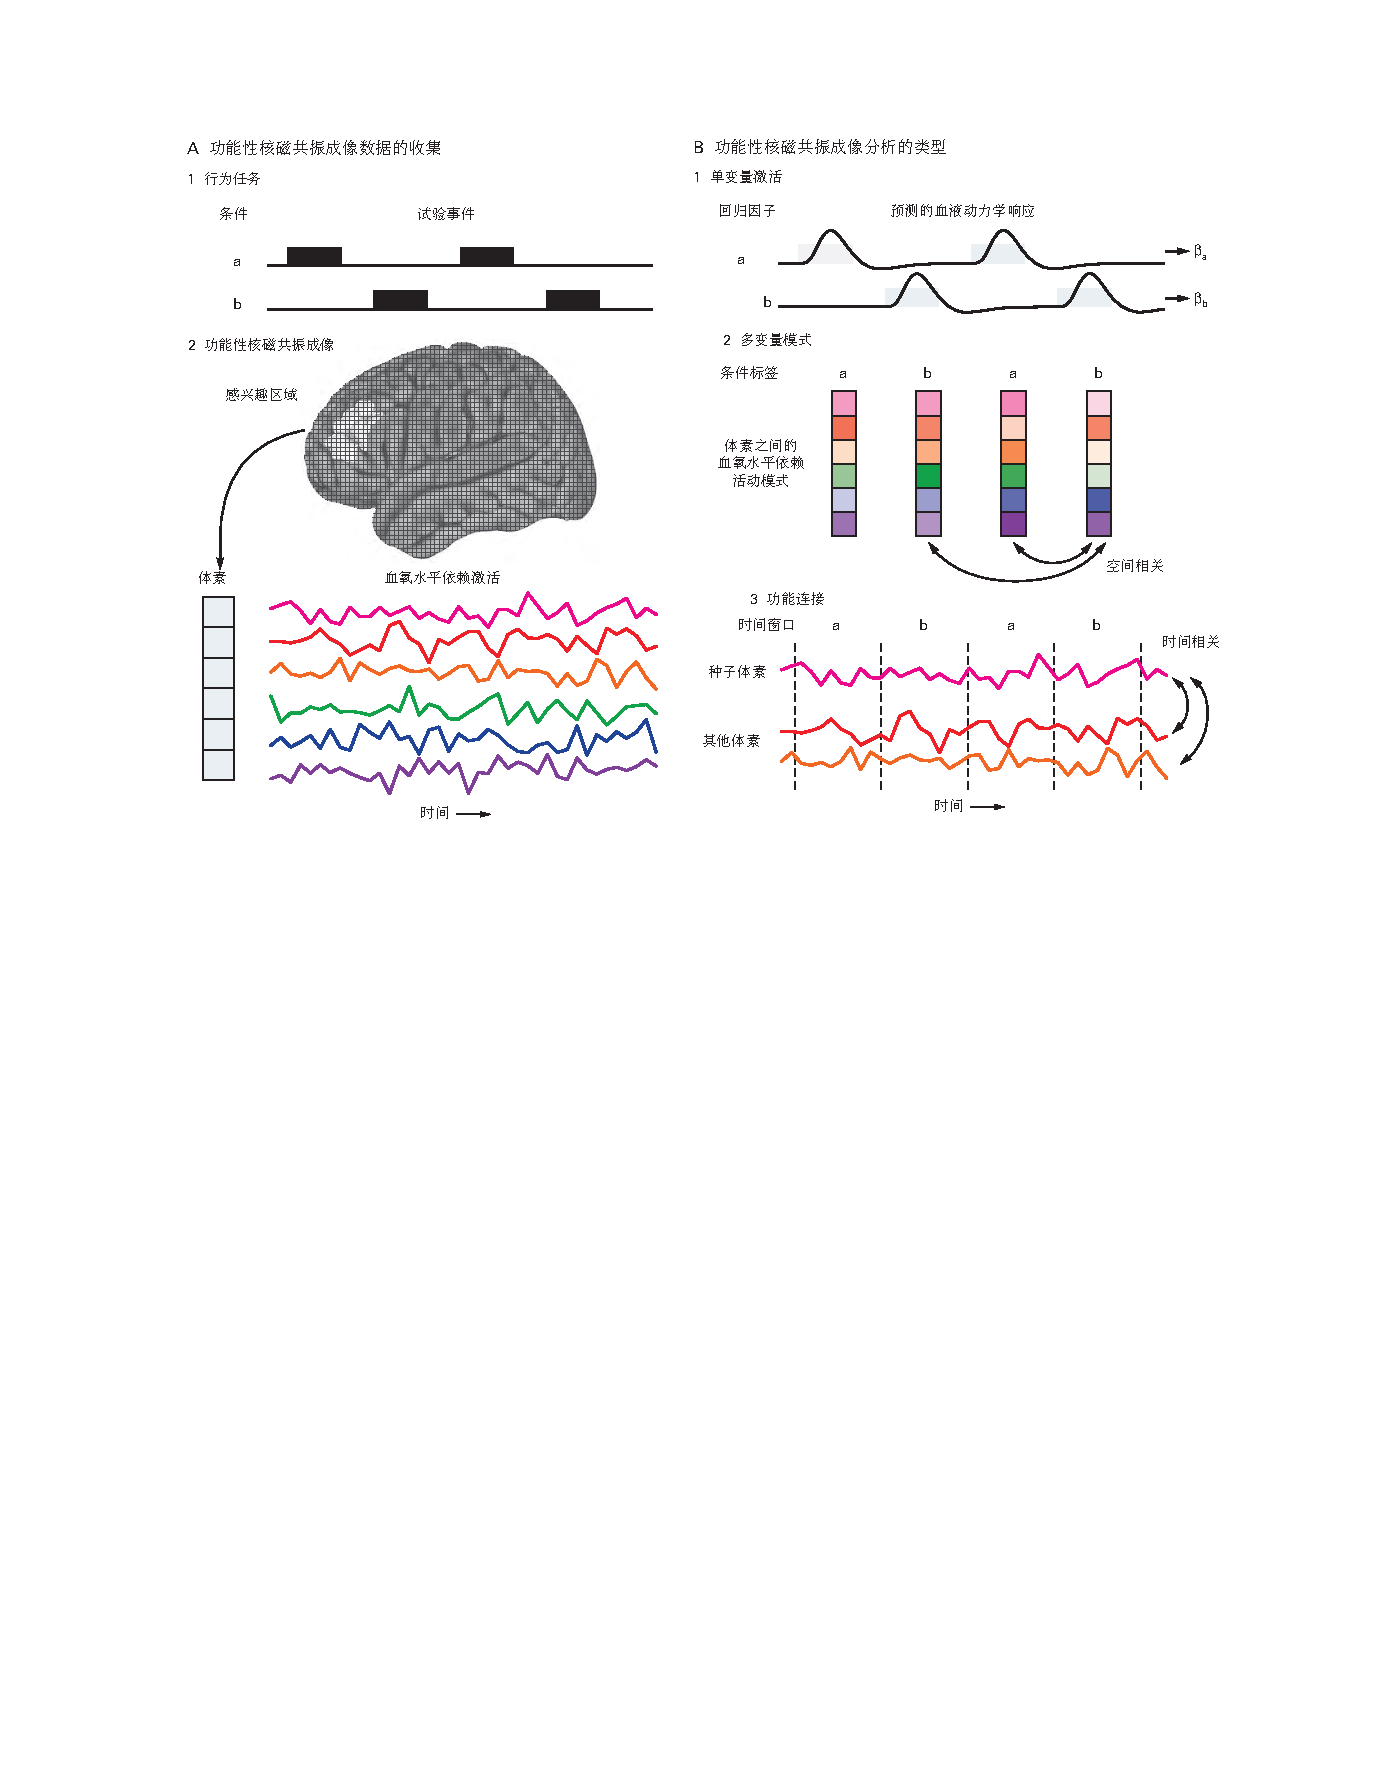
\includegraphics[width=1.0\linewidth]{chap06/fig_6_2}
	\caption{收集和分析\textit{功能性磁共振成像}数据。 
		\textbf{A.} 功能性核磁共振成像实验通常涉及受试者执行行为任务,同时从大脑测量血氧水平依赖活动。
		1. 示例任务包含两个在时间上交替出现的条件(a, b),每个条件都描绘了两个事件(黑色矩形)。
		2. 在任务期间,来自感兴趣区域的六个示例体素(不同颜色)中\textit{血氧水平依赖}活动的时间进程。 
		分析通常侧重于大脑中的感兴趣区域或其他体素子集,以减少执行的统计测试的数量。
		当分析大脑中的所有体素时,应用统计校正来减少误报的数量。
		此类分析的结果通常作为颜色编码的热图叠加在结构\textit{核磁共振成像}上。
		该图是广泛预处理和分析的结果,并不直接反映神经元活动甚至血液氧合。
		相反,体素是彩色的,以表明它们已经超过了在统计测试中被认为是重要的阈值。
		\textbf{B.} 功能性核磁共振成像实验中经常使用三种分析方法,例如 A 中描述的方法。
		1. 单变量激活分析试图根据任务中发生的情况来解释每个体素的血氧水平依赖活动。 
		这是使用统计模型完成的,该模型包含每个任务条件的回归变量,指定从该条件(灰色矩形)开始的试验事件的预测血液动力学响应(钟形曲线)。 
		将模型拟合到血氧水平依赖活动的结果是每个体素中每个回归量的$\beta$值,量化体素对该条件试验的平均响应。 
		可以减去体素的$\beta$值以衡量在一种情况下是否比另一种情况下有更大的响应。
		为了确定统计显著性,比较了受试者之间每个体素中条件之间激活的差异。
		2. 多变量模式分析考虑了跨体素的血氧水平依赖活动模式。
		这些空间模式是为每个试验从体素的一个子集(描绘了六个)中提取的,并且在特定时刻,通常是预测的血液动力学响应的峰值(颜色饱和度表示该试验中每个体素中 血氧水平依赖活动的幅度)。
		有两种常见的分析这些模式的方法。
		第一个(如图所示)涉及计算来自一对试验的模式的空间相关性,以探索体素对试验的反应有何相似之处。
		如果一个大脑区域代表不同条件下的不同信息,那么对于来自相同条件和不同条件的成对试验,这种模式相似性应该更高。
		第二种类型的多元模式分析(未显示)使用一种称为模式分类的机器学习。
		一些模式及其相应的条件标签用于训练分类器模型,根据它们在区分条件时的有用程度为体素分配权重。
		然后使用未训练的其他模式对该模型进行测试。
		如果大脑区域代表不同条件下的不同信息,则模型应该能够正确猜测从哪种条件下提取模式。
		为了确定统计显著性,一个区域中的空间相关性或分类准确度会在受试者之间进行比较。
		3. 功能连通性分析检查血氧水平依赖活动如何随时间在体素之间相关。
		通常,选择种子体素或感兴趣区域,其时间进程(粉红色曲线)与其他体素的时间进程(此处显示两个)相关。
		这可以在受试者休息时执行,从而产生每个体素的相关值,可用于识别基线状态下的大脑网络。
		功能连通性也可以在任务的不同时间窗口(虚线)中计算,从而为每个试验生成一个相关值,可用于了解这些网络的动态。
		为了确定统计显著性,每个体素的时间相关性在条件之间或与零之间在受试者之间进行比较。}
	\label{fig:6_2}
\end{figure}

% β也就是beta,代表回归系数,标准化的回归系数代表自变量也就是预测变量和因变量的相关



\subsection{功能性核磁共振成像数据首先需要通过以下预处理步骤准备分析}

在分析数据之前,必须为处理做好准备。 
这是通过一系列称为预处理的步骤完成的。 
预处理旨在消除数据中由受试者或核磁共振成像机器引起的已知噪声源。 
标准实践包括五个基本步骤,称为运动校正、切片时间校正、时间过滤、空间平滑和解剖对齐。


\textit{运动校正}旨在解决由于主体头部运动而导致的数据中不可避免的噪声。
即使是最好的受试者也会在扫描过程中将头部移动几毫米,这样横跨三维脑体积的体素就会变得有些错位。
可以使用空间插值算法纠正此移动,该算法在每次运行中排列所有卷。
该算法量化扫描期间每个点的移动量,包括 $x$、$y$ 和 $z$ 维度的平移,以及围绕这些轴(分别为俯仰、滚动和偏航)的旋转量。
这六个时间课程稍后可以作为回归器包含在数据分析中,以进一步消除运动伪影。


应用\textit{切片时间校正}来处理跨不同切片的样本采集时间的差异。
\textit{平面回波成像}序列按顺序收集构成每个脑容量的切片,通常以交错顺序进行,以避免相邻切片的污染。
因此,同一体积的第一个和最后一个采集切片的时间存在很大差异,它们在时间上分别更接近于前一个体积和后一个体积,而不是相互之间。
可以通过时间插值来完成对切片时间差异的校正,以估计如果同时获取所有切片时信号会是什么。


\textit{时间滤波}和\textit{空间平滑}旨在提高信噪比。
\textit{时间滤波}去除了每个体素中时间过程的组成部分,这些组成部分很可能是噪声而不是有意义的方差,例如通常由扫描仪漂移引起的非常低的频率(> 100 秒周期)。 
\textit{空间平滑}应用内核(通常为 4-8 毫米宽)来模糊单个体积,平均掉相邻体素之间的噪声,并提高功能在解剖对齐后跨对象重叠的几率。


这种\textit{解剖对齐}是通过将跨运行和受试者的数据注册到标准模板(例如蒙特利尔神经病学研究所或\textit{塔莱拉什空间})来完成的,通常使用简单的转换(例如,移位、旋转、缩放)。
通常,功能性核磁共振成像数据首先与来自同一主题的结构扫描对齐,然后将此结构扫描与标准模板对齐。


完成这五个步骤后,数据就可以进行分析了。



\subsection{功能性核磁共振成像可用于将认知功能定位到特定的大脑区域}

第一种功能性核磁共振成像分析旨在\textit{定位}大脑中的功能并确定哪些大脑区域与行为相关。 
这是基于让受试者在功能性核磁共振成像期间完成一项任务,然后检查实验不同阶段与大脑不同部位血氧水平依赖 活动变化之间的关系。 
根据研究人员对实验中不同时间发生的情况的了解,可以推断出这些区域的功能。


执行一系列统计分析来量化这种关系并确定其重要性。 
通常,这是使用称为广义线性模型的统计回归方法来完成的。 
广义线性模型试图将观察到的数据(这里是每个体素中 血氧水平依赖活动的时间过程)解释为反映独立变量(例如,任务条件)和协变量(例如,运动参数)的回归量的线性组合。


模拟任务条件的回归变量可以作为一个假设,假设体素参与该任务操纵的认知功能时应该如何响应。
每个条件的回归量是通过在实验时间线中标记该条件的每次试验的开始和持续时间来生成的,对应于预期的神经元活动,然后考虑延迟的血液动力学反应。
所有回归量同时适合每个体素中的功能性核磁共振成像活动,结果是每个条件和体素的参数估计(或$\beta$),反映了该条件对 平均的。


为了定位一个函数,来自两个或多个条件的$\beta$被对比比较。 
最基本的对比形式是从另一个(例如,实验条件)中减去一个$\beta$(例如,控制条件)。 
对比度通常是每个受试者运行的平均值,然后进入 $t$ 检验以评估受试者之间的可靠性。 
因为统计数据是针对每个体素计算的,所以存在高的误报风险,并且需要对多重比较进行校正(例如,如果体素与其他重要体素聚集在一起,则通过给予体素更多的信任)。 
或者,可以执行更受约束的分析,重点关注先验定义的有限数量的感兴趣区域。 
然后可以对感兴趣区域中的体素取对比度值的平均值以生成区域估计,而不是检查大脑中的所有体素,从而减少比较次数。


这种一般的方法系列通常被描述为测量单变量激活(“单变量”是因为每个体素或区域都是独立处理的),而“激活”是因为结果是衡量一种情况相对于另一种情况引起的相对活动。
这种分析通常用于将认知功能定位到大脑中的一组体素或区域。


然而,单变量激活不仅仅用于定位。
例如,\textit{广义线性模型}可以根据实验参数(例如,工作记忆负荷)、行为测量(例如,响应时间)为回归量中的每个试验分配连续权重而不是分类权重,从而对血氧水平依赖 活动进行定量预测 ),或计算模型(例如,强化学习中的预测误差)。
生成的$\beta$反映了体素与感兴趣变量的相关程度。


单变量激活的另一个用途是测量\textit{血氧水平依赖}活动的变化作为重复刺激的函数。
这些研究利用了适应(或重复抑制):
刺激选择性神经元对重复刺激和新刺激的反应较少的趋势。
这一事实允许通过进行相关和不相关刺激按顺序呈现的实验来推断大脑区域的调整。
在一些试验中,一个刺激之后是几乎重复的相同刺激,但特征发生了变化(例如,它的位置或大小)。
单变量分析测试这些试验中来自该区域的体素的血氧水平依赖活动是否低于其他试验,其中
(1)第一个刺激之后是不相关的第二个刺激,或者
(2)改变的刺激之前是不相关的刺激。
如果观察到这样的血氧水平依赖减少,则该区域可以解释为未针对更改的特征进行调整(例如,该区域可以被认为是位置或大小不变的)。


% 解码
\subsection{功能性核磁共振成像可用于解码大脑中所代表的信息}

第二类功能性核磁共振成像分析旨在描述大脑不同区域代表的信息类型以指导行为。
这些分析不是独立分析体素或对感兴趣区域内的体素进行平均,而是检查多个体素上血氧水平依赖活动的空间模式所携带的信息。 
这通常称为\textit{多元模式分析}。
根据活动模式的相似性或分类,有两种类型的\textit{多元模式分析}。


基于相似性的\textit{多元模式分析}试图了解大脑区域中包含或“表示”了哪些信息。 
这是通过检查该区域在实验中处理不同条件或刺激的相似程度来实现的。 
这种相似性是根据感兴趣区域中跨体素的激活模式计算的,定义为来自广义线性模型的$\beta$值模式或来自预处理数据的原始血氧水平依赖活动模式。 
一旦为多个条件或刺激定义了这些模式,就会计算每对模式的相关性或距离。 
这会生成感兴趣区域内条件或刺激之间的成对相似性矩阵。 
使用此矩阵,可以推断出感兴趣区域对哪些信息最敏感。 
例如,如果向受试者展示不同物体(例如,香蕉、独木舟、出租车)的照片,则可以为不同的大脑区域计算由这些物体引起的活动模式之间的距离矩阵。
香蕉和独木舟之间的距离小于它们与出租车之间的距离的\textit{感兴趣区域}可以解释为表示该区域代表形状(即凹面);
香蕉和出租车之间距离最短的另一个区域可能代表颜色(即黄色);
或者独木舟和出租车之间距离最短的一个可能被解释为代表功能(即交通)。


功能性核磁共振成像的神经相似性也可以与以其他方式计算的相同条件或刺激的相似性进行比较,包括人类判断、计算模型或其他物种的神经测量。
例如,如果人类受试者根据彼此看起来的相似程度对大量刺激进行评分,则具有匹配相似结构的大脑区域可被视为该行为的候选来源。
这种计算神经和行为相似性矩阵之间或来自两个来源的神经相似性矩阵之间的二阶相关性的方法称为\textit{表征相似性分析}。


基于分类器的\textit{多元模式分析}使用机器学习技术(在第~\ref{chap:chap5}~章中讨论)来解码大脑区域中存在的信息。 
第一步是在功能性核磁共振成像数据的子集上\textit{训练分类器}模型,以区分条件或刺激类别与感兴趣区域中跨体素的 血氧水平依赖活动模式。
这些模式通常是从个别试验中获得的,每个试验都根据相应试验的条件或刺激进行标记。
因此,该训练集包含每个类别的几个大脑模式示例。
分类器训练可以使用许多不同的算法,最常见的两种是\textit{支持向量机}和\textit{正则化逻辑回归}。
结果通常是每个体素的权重,反映了该体素中的活动如何与其他体素一起对分类做出贡献。
训练后的第二步是\textit{测试}分类器,方法是检查分类器从 功能性核磁共振成像数据的保留和独立子集中解码模式的能力(例如,来自不同的运行或受试者)。
每个测试试验中血氧水平依赖活动的模式乘以学习到的分类器权重并相加以产生关于模式应该如何标记的猜测。
分类准确度被量化为这些猜测与正确标签相匹配的比例。
重要的是,这种方法可用于了解不同的大脑区域如何产生行为,例如通过尝试对执行的动作、做出的决定或检索的记忆进行分类。



% 预测
\subsection{功能性核磁共振成像可用于测量大脑网络中的相关活动}

第三类功能性核磁共振成像分析旨在了解大脑作为网络的组织。
了解大脑区域单独做什么并不能完全解释大脑作为一个整体是如何产生行为的。
了解大脑区域如何相互关联也很重要,也就是说,一个区域的输入从哪里来,输出到哪里?
这需要了解哪些区域相互通信以及它们何时以及如何传输信息。
这很难用功能性核磁共振成像明确确定,但可以通过测量随时间变化的体素或区域之间 血氧水平依赖活动的相关性来估计。
如果大脑的两个部分有相关的活动,它们可能共享相同的信息或参与相同的过程。
这种相关性被解释为功能连通性的度量。


使用功能性核磁共振成像研究功能连接的一种方法是测量静息状态下的血氧水平依赖相关性。 
在受试者静止不动而不执行任务时对其进行扫描,然后提取来自一个“种子”感兴趣区域的血氧水平依赖活动的时间进程,并将其与来自其他感兴趣区域或大脑中所有体素的时间进程相关联。
或者,可以在没有种子的情况下使用聚类或成分分析来识别具有相似时间分布的体素集合。
以这些方式定义的静息功能连接有助于揭示大脑包含多个大型区域网络。
这些网络中研究最广泛的称为默认模式网络,包括后内侧皮层、外侧顶叶皮层和内侧前额叶皮层。
根据定义,静止连接不能与并发行为相关联。
它也不是静态的,因为告诉受试者不要做任何事情并不会限制他们的想法。
然而,通过检查它在疾病或失调中如何出错以及它如何与人之间的认知差异相关,可以间接地将静息连接与行为联系起来。


如果在任务期间而不是在休息时测量功能连通性,则可以更直接地将其与行为联系起来。 
解释区域之间这种相关性的一个困难是,两个区域在任务期间可能相关,不是因为它们相互通信,而是因为第三个变量。
例如,这些区域可能独立但同时对同一刺激做出反应。
因此,基于任务的功能连接通常是在删除或以其他方式考虑由刺激引起的血氧水平依赖反应后计算的。 
这种方法允许通过实验操作功能连接,并在不同任务条件下进行比较。
这些比较提供了对网络中大脑区域的参与和交互如何动态变化以支持不同行为的洞察力。
这已被证明有助于理解注意力、动机和记忆等认知功能,这些功能取决于某些大脑区域对其他区域的调节。


功能连接也可以被视为一种模式(相关性而非活动)并提交给\textit{多元模式分析}。 
相关模式比活动模式规模更大:
如果活动模式中有 $n$ 个体素,则相关模式中大约有 $n^2$ 个体素对。
因此,使用图论总结相关模式的属性可能会有所帮助,其中单个体素或区域被视为图中的节点,这些节点之间的功能连接决定了边缘强度。



\section{功能性核磁共振成像研究带来了基本的见解}

功能性核磁共振成像改变了我们对人类行为的基本神经生物学构建块的理解。
将认知心理学的实验操作和计算模型与精确的神经生物学测量相结合,扩展了现有的心智和大脑理论,并激发了新的想法。
功能性核磁共振成像的发现不仅影响了我们对被认为是人类特有行为的理解,还影响了长期以来在动物身上研究的行为。


在本节中,我们回顾了这一进展的三个例子。 
\textit{面部感知}研究揭示了人类核磁共振成像研究如何启发了动物研究。
\textit{记忆}研究说明了功能性核磁共振成像如何挑战认知心理学和系统神经科学的理论。
\textit{决策}研究展示了动物研究和计算模型如何推动功能性核磁共振成像研究。


\subsection{人类的功能性核磁共振成像研究启发了动物的神经生理学研究}

在过去的二十年里,我们对大脑如何感知面孔的理解有了长足的发展(第~\ref{chap:chap24}~章)。 
下面描述的进展提供了一个例子,说明人类功能性核磁共振成像的发现如何激发了对非人类灵长类动物进行神经元记录和因果干预的后续研究。
这种跨物种和跨技术的协同作用使人们对面孔识别的基本过程有了更全面的了解。


某些类别的刺激比其他类别的刺激对生存更重要。 
大脑是否有专门的机制来处理这种刺激? 
人脸是一个明显的例子。 
功能性核磁共振成像的发展与仔细和系统的实验设计相结合,导致了对人脑中面部处理方式和位置的重要见解。 
梭状回中的一个区域,通常被称为\textit{梭状回面孔区},被发现在人类观察面部时表现出强烈和选择性的 血氧水平依赖活动。


导致这一发现的早期功能性核磁共振成像研究依赖于简单的设计,在这些设计中,受试者被呈现了一系列不同类型的视觉刺激。
为了测量大脑区域的面部选择性,将对面部的血氧水平依赖反应与对其他类别(例如,地点、物体)的血氧水平依赖反应进行比较。 
外侧梭状回的一个区域,最可靠地位于右半球,被面部强烈激活。
这些发现与早期对非人类灵长类动物中对面部有反应的单个神经元的发现相吻合,但激发了新一轮的动物研究浪潮,以检查更大规模的大脑区域网络。
这些较新的动物研究借鉴了人类研究的实验设计,首先使用功能性核磁共振成像寻找\textit{梭状回面孔区}的同源物。
然后用神经元记录和刺激侵入性地探测由此产生的面部贴片。
这揭示了对灵长类动物面部处理的分布式神经回路的洞察。


除了选择性地响应面部刺激之外,\textit{梭状回面孔区}是否有助于面部识别行为? 
这个问题已经通过使用已知会影响面部识别的刺激变化(例如,呈现倒置的面部或呈现面部的一部分)来解决。 
最初的功能性核磁共振成像研究使用刺激类别(倒置与直立的面部)的简单比较产生了微弱和混合的结果。
后续研究使用适应设计来确定当面部重复完整或改变时 血氧水平依赖活动如何变化。
研究结果表明,\textit{梭状回面孔区}代表完整的面孔与以破坏行为识别的方式重新配置相同的视觉特征时不同。


检查一个区域的行为意义的另一种方法是研究\textit{有行为缺陷}的患者。
在这种情况下,面部识别障碍被称为\textit{面容失认症}。
令人惊讶的是,一些功能性核磁共振成像研究在这些患者中发现了完整的梭状回,这让人怀疑它对面部感知的必要性。 
然而,这里也使用适应设计的后续研究证明了信息:当重复相同的面孔时,面容失认症的其他完整的梭状回不适应。 
这表明梭状回在面容失认症患者中的反应不同,与其对面部识别的重要性一致。


视觉类别或更普遍的心理过程可以映射到像梭状回这样的一个或少数区域,这一发现对于思考思维与大脑之间的关系非常重要。
特定功能是局部化的还是广泛分布的一直是整个神经科学史上关于大脑组织的核心问题(第 ~\ref{chap:chap1}~章)。 
梭状回和面部贴片系统的发现提供了定位的新证据,并鼓励研究人员追寻其他复杂认知功能可能定位于特定大脑区域或小型节点集的假设,但也质疑定位是否正确思考大脑组织的方式。
例如,进一步的研究表明,人脸在视觉皮层上产生广泛分布的反应,梭状回可以被用来识别我们拥有专业知识的其他种类的物体。
这些争论反映了这项原创作品的变革性质,既适用于人脑研究,也适用于动物模型中的相关问题。



\subsection{功能性核磁共振成像研究挑战了认知心理学和系统神经科学的理论}

许多认知心理学的理论模型最初对大脑是不可知论的。 
然而,现在有几个功能性核磁共振成像发现的例子改变了我们对认知的组织和机制的理解。


一个突出的例子是对\textit{记忆}的研究。
从 19 世纪开始,记忆研究的总体目标是了解记忆是如何创建、检索和使用的,以及这些过程是否因记忆类型而异。 
一项重要发现来自对患者\textit{亨利$\cdot$莫莱森}的研究。 
认识到海马体受损会导致丧失形成新\textit{自传式记忆}的能力,但不会影响学习某些技能的能力(第~\ref{chap:chap52}~章)。
这些发现导致了这样的想法,即记忆可以分为两大类,有意识的和无意识的(也称为陈述性与程序性或显性与隐性)。
在定位的传统中,这些和其他类型的记忆被映射到不同的大脑区域,基于患者大脑中受损的位置以及他们表现出的行为症状。


后来对健康人脑的功能性核磁共振成像研究有助于揭示这种二分法过于简单化了。
首先,一些使用后来被称为后续记忆任务的研究表明,海马体以外的区域与陈述性记忆的成功形成有关。
在此类研究中,受试者在扫描时会收到一系列刺激(图片或文字)。
之后,通常在核磁共振仪之外,测试他们对这些刺激的记忆。
刺激最初被编码时的血氧水平依赖反应然后根据它随后是被记住还是被遗忘来排序。
将这些条件进行对比以揭示在成功的记忆形成过程中哪些大脑区域表现出更多(或更少)的活动。
除了在海马体和周围的内侧颞叶中发现这种差异外,前额叶和顶叶皮层中的血氧水平依赖活动也可以预测后期记忆。 
通过测量健康个体的整个大脑,功能性核磁共振成像揭示了陈述性记忆由不止一个大脑系统提供,与前额叶皮层(例如,语义阐述)和顶叶皮层(例如,选择性注意)相关的过程也参与编码。


功能性核磁共振成像研究以另一种方式挑战了传统的记忆组织分类学。
功能性核磁共振成像显示,以前假设不涉及海马体(或陈述性记忆)的范围广泛的任务实际上确实始终与该区域有关。
这些研究通常使用通常被认为是无意识的学习任务,在这些任务中,受试者有机会学习但从未被要求报告他们的记忆,并且在某些情况下,如果提示则无法这样做。
例如,在概率分类任务中,受试者通过反复试验学习将\textit{视觉提示}分类,即使线索和类别之间的关系有时不可靠。
估计此类学习试验期间的血氧水平依赖活动,并将其与不涉及试错学习的基线任务(例如,研究线索及其提供的类别)进行比较。
这种比较通常揭示了纹状体的激活,但也可靠地揭示了海马体的激活(见第~\ref{chap:chap52}~章)。


总之,功能性核磁共振成像研究被认为依赖于陈述性记忆的任务通常会招募海马体以外的区域,而被认为依赖于程序性记忆的任务可以招募海马体。
在这两种情况下,这些发现都是偶然的,并且之所以成为可能,只是因为数据是通过功能性核磁共振成像从整个大脑中获得的。
尽管这些开始时是意想不到的结果,但它们导致了系统的后续研究,更新了我们对记忆组织的理解。
主要是,他们挑战了最初强调有意识的意识作为海马体处理的决定性特征。
这反过来又有助于将人类研究的结果与动物研究的结果联系起来,在动物研究中,有意识记忆的概念不太重要,而海马体参与的任务通常涉及空间导航。
因此,\textit{功能性磁共振成像}在人类身上的发现已经改变了我们对记忆理论模型的理解,包括神经结构和认知行为。



% 决策
\subsection{功能性核磁共振成像研究检验了动物研究和计算模型的预测}

计算模型与功能性核磁共振成像的集成一直是认知神经科学的重要发展。
这方面的一个例子来自对大脑如何\textit{学习预测}和\textit{获得奖励}的研究,以及将这一过程形式化的\textit{强化学习模型}。
这些模型与基于奖励的动物决策研究共同进化,这也启发了后来的人类研究。


这些研究和理论的核心是,中脑多巴胺能神经元会增加它们的放电以响应意想不到的奖励,例如果汁(第 ~\ref{chap:chap43}~章)。 
一旦预测性线索与奖励可靠地配对,神经元就会及时将它们的反应转移到这个预测性线索上。
如果预测的奖励没有发生,则激活会减少。
这种反应模式表明中脑多巴胺能神经元发出预期奖励与实际奖励之间差异的信号。
这种差异通常被称为奖励预测误差,并且已使用基于强化学习理论的方程式进行建模。
当该模型应用于涉及奖励的人工任务时,可以在逐个试验的基础上估计假设的奖励预测误差。
然后,这些估计可用于预测血氧水平依赖活动并识别可能参与人脑强化学习的体素和区域。


在此类典型研究中,受试者在功能性核磁共振成像期间执行学习任务,做出一系列关于\textit{视觉提示}的选择以预测可能的奖励。
他们在每次选择后立即了解结果。
例如,受试者可能会看到两种形状(例如,圆形、三角形),通过按下按钮选择一种形状,然后了解该选择是否会带来金钱奖励。
此类任务的关键特征是形状和奖励之间的关联是概率性的,并且会在实验过程中发生变化。
由于这种嘈杂的关系,受试者必须学会跟踪每种形状的奖励可能性。
可以根据受试者选择和奖励的历史计算每次试验的奖励预测误差,然后将其包含在对其功能性核磁共振数据的分析中。
许多使用这种方法的研究发现,逐个试验的奖励预测误差与腹侧纹状体中的血氧水平依赖活动相关,腹侧纹状体是一个接收中脑多巴胺能神经元输入的区域。


其他计算模型,如整合了认知心理学、计算机科学和神经科学的深度神经网络,也通过产生关于大脑活动的新假设发挥了重要的理论作用。
由于这些模型通常受到大脑结构和功能的启发,因此它们有助于弥合分析水平,从动物的生理记录到人类的功能性核磁共振成像。 
它们还通过模拟可以在大脑中寻找的心理和神经生物学兴趣变量,在数据分析中发挥有用的作用,这种方法通常被称为基于模型的分析。



\section{功能性核磁共振成像研究需要仔细解读}

前面提供的例子说明了功能性核磁共振成像如何提高我们对大脑和行为之间联系的理解。 
在与心理学的接口上,功能性核磁共振成像可以补充纯粹的行为测量。
许多复杂的人类行为(例如,记忆回忆、决策制定)取决于多个处理阶段和组件。
与仅基于简单的行为测量(例如准确性或响应时间)的行为相比,使用功能性核磁共振成像测量这些过程可以提供更丰富、更机械的行为解释。
在与系统神经科学的接口上,功能性核磁共振成像补充了直接神经元记录。
大多数大脑区域(例如,海马体)支持多种行为,并且与其他区域协调一致。
使用功能性核磁共振成像对整个大脑进行成像的能力使得在网络层面更全面地了解神经机制成为可能。


那么在任务期间在某个区域发现血氧水平依赖活动意味着什么?
大脑和行为之间映射的多样性对功能性核磁共振成像结果的解释提出了严峻挑战(图~\ref{fig:6_3})。
一个基本的考虑因素是推理的类型。 
大多数功能性核磁共振成像研究使用前向推理,其中一项实验比较了操纵特定心理过程参与的任务条件之间的 血氧水平依赖活动(例如,比较面部与非面部刺激的影响以研究面部识别)。
可以推断这些条件不同的大脑区域参与了操纵过程。
前向推理依赖于任务操作,因此允许研究人员推断大脑活动的差异与感兴趣的心理过程有关。


\begin{figure}[htbp]
	\centering
	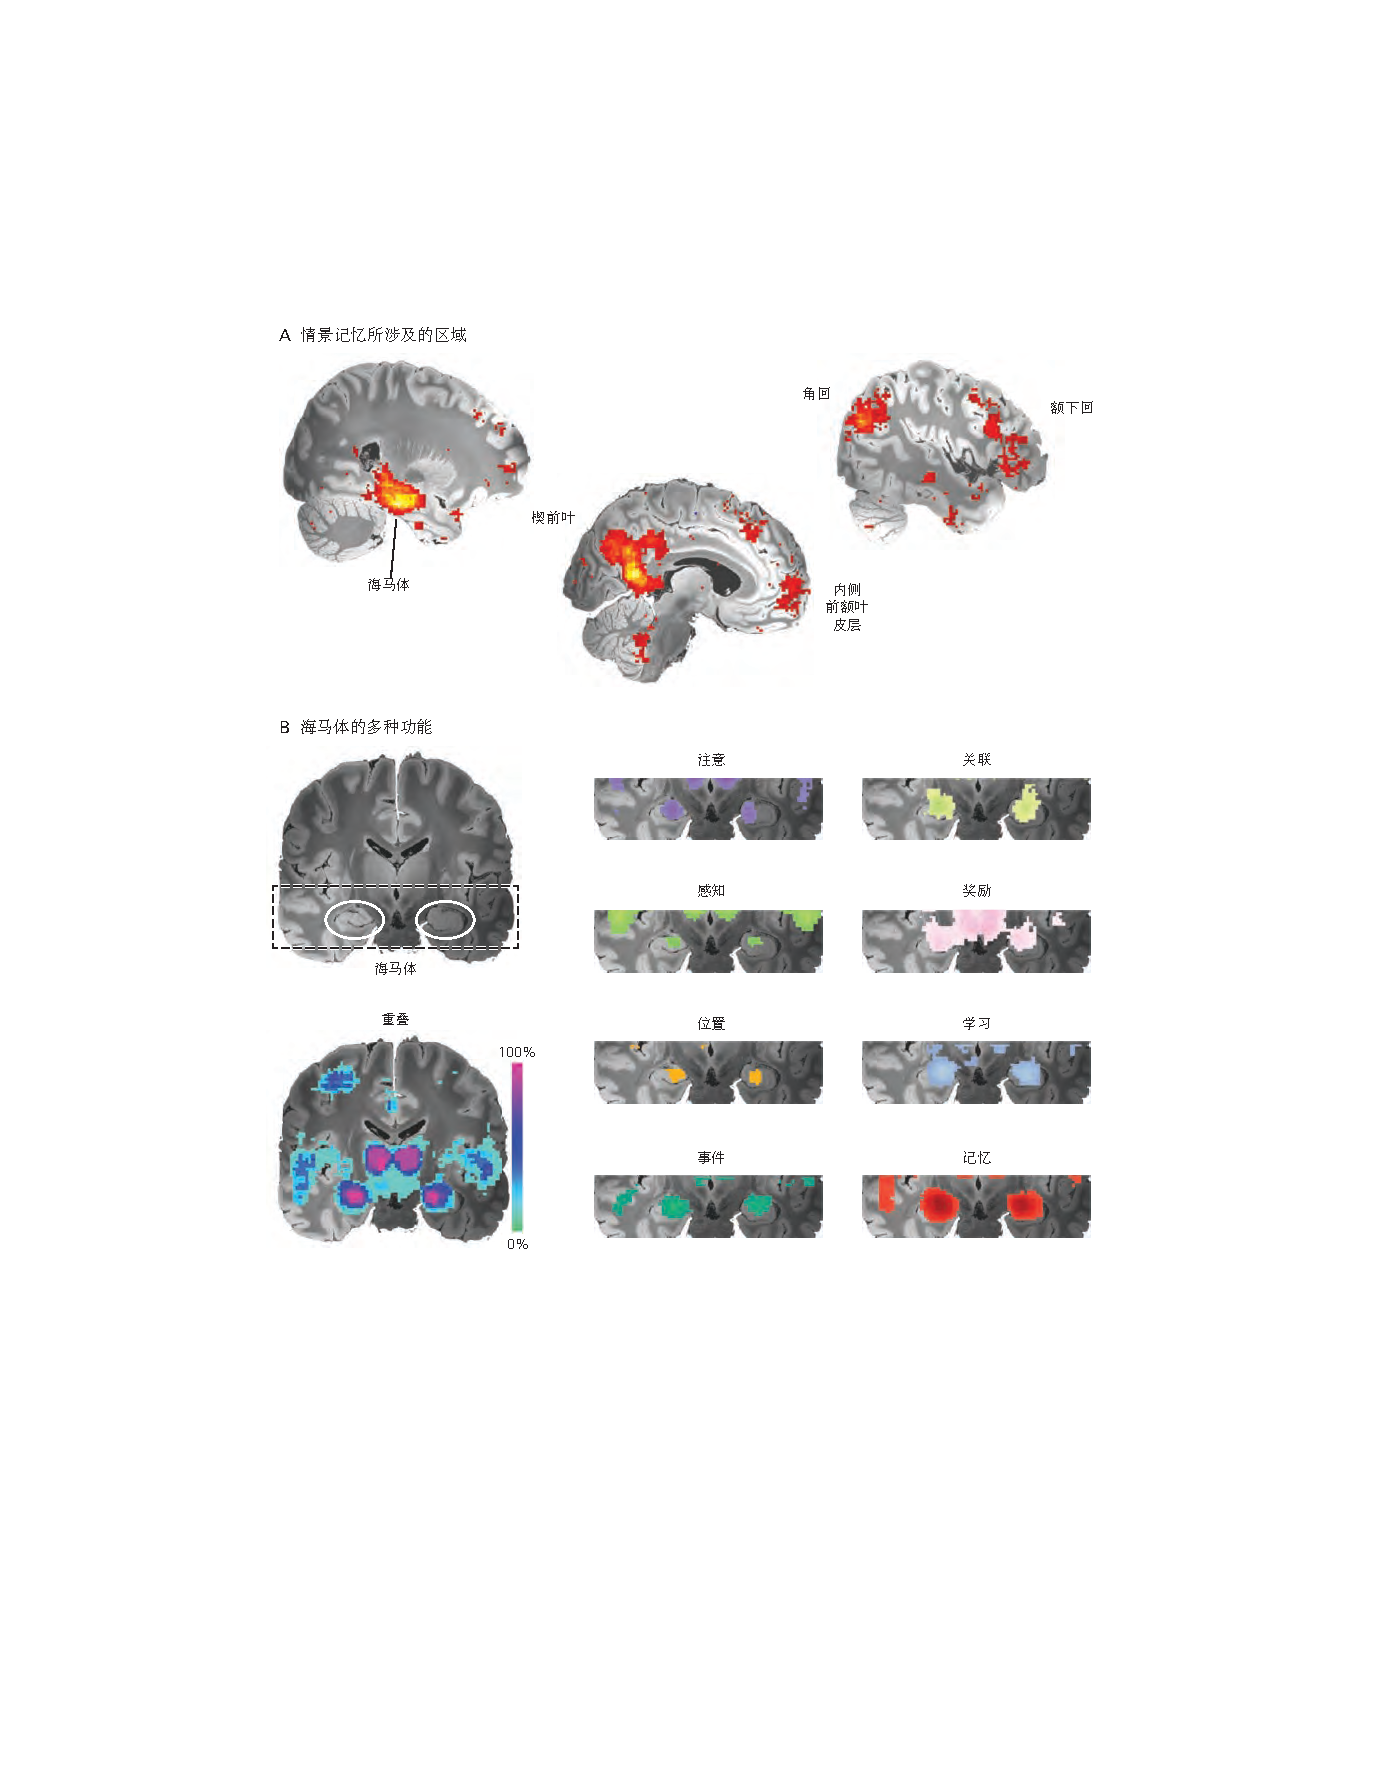
\includegraphics[width=1.0\linewidth]{chap06/fig_6_3}
	\caption{映射思维和大脑的挑战。
		对\textit{功能性核磁共振成像}数据的任何解释都必须考虑认知功能与大脑区域之间关系的复杂性。
		此处通过来自包含 14,000 多项已发表的\textit{功能性核磁共振成像}研究数据库的\textit{元分析}来说明这种复杂性。
		\textbf{A.} 这张地图显示,多个大脑区域参与\textit{情景记忆},即对过去特定事件的编码和检索。
		彩色体素表明在报告这些体素激活的研究中术语“偶发性”的可能性很高(反向推理)。
		这个例子说明了\textit{单个认知功能}如何与\textit{多个大脑区域}相关联(一对多映射)。
		\textbf{B.} 这些图显示海马体参与了多种认知功能(每个半球的白色圆圈)。 
		每个插图大脑中的彩色体素表明这些体素在检查相应术语(前向推理)的研究中被激活的可能性很高。
		重叠图显示了激活每个体素的这些术语的百分比。
		这个例子说明了\textit{单个大脑区域}如何与\textit{多个认知功能}和行为相关联(多对一映射)。}
	\label{fig:6_3}
\end{figure}


% 神经活动 (反向)->心理活动
通过反向推理,神经活动的差异是推断哪个特定心理过程活跃的基础,即使导致差异的条件并非旨在操纵该过程。 
例如,在之前的人脸与非人脸对比中,研究人员可能会将纹状体中的不同活动解释为人脸有益的证据。
这种反向推理通常是不合理的,因为奖励既没有被测量也没有被操纵,即解释是基于其他操纵奖励并发现纹状体活动的研究。
问题的出现是因为每个大脑区域通常支持不止一种功能,这意味着仅通过观察活动就不清楚哪些功能参与了。
事实上,纹状体也与运动密切相关,所以也许面部参与运动而不是奖励过程?
这个例子中逻辑合理的结论反映了前向推理,即纹状体参与了面部识别的某些(尚未解决的)方面。


因此,一种解决方案是不在功能性核磁共振成像研究中使用反向推理。
然而,在某些情况下,反向推理可能是可取的,甚至是必要的。
例如,反向推理可以让研究人员进行探索性分析并生成新的假设,甚至可以从为其他目的收集的数据中得出。
这对于充分利用难以收集的功能性核磁共振成像数据尤其重要,例如来自儿童、老人和患者的数据(方框~\ref{box:6_2})。
出于这种需要,已经开发了统计工具来支持反向推理。
例如,基于网络的工具 Neurosynth 使用已发表研究的大型数据库来分配特定心理过程(例如奖励)的概率,因为在特定区域(例如纹状体)中观察到了血氧水平依赖活动。


\begin{proposition}[现实世界中的大脑成像] \label{box:6_2}
	
	\quad \quad 利用非侵入性工具对人脑进行成像和测量内部心理过程的能力引起了人们对将功能磁共振成像应用于各种现实世界问题的兴趣,如临床诊断和治疗、法律和司法、人工智能、营销和经济以及政治。
	
	\quad \quad 在临床领域,一个有趣的方向是使用功能磁共振成像来检查植物人状态的患者。
	研究表明,一些这样的患者表现出反映心理处理的大脑活动。
	例如,患者可能表现为昏迷(无意识、非交流和对外部刺激不反应),但当被要求思考一个动作时,运动皮层或当被要求想象特定的\textit{视觉提示}时,在特定类别的视觉区域表现出神经活动。
	这些发现可能会影响临床医生对患者的预后和治疗。
	
	\quad \quad \textit{功能性核磁共振成像}在现实世界中的另一个潜在应用是测谎。
	根据大脑活动准确区分真相和谎言的能力在法庭上可能具有重要价值。
	一些实验室研究报告称,当一组受试者被要求重复撒谎时,大脑活动会有所不同。
	然而,为了有用,功能磁共振成像需要以一种不受策略或对策影响的方式,提供高度可靠的证据,证明一个人是否在特定事件上撒谎。
	这在目前是不可能的,事实上,功能磁共振成像的证据在法庭上通常是不可接受的。
	
	\quad \quad 功能磁共振成像的这些和其他应用引起了道德和隐私方面的担忧。
	例如,当局可以使用功能磁共振成像数据来证明相应的决定(如有罪或无罪),利用公众的偏见来相信生物学解释,即使基础科学尚未确定。
	更令人不安的是,人类目前对我们是否分享内心想法和感受拥有自主权,但感知这些信息的设备可能会改变这一点。
	因此,神经科学家在考虑实际应用时面临的一个重要挑战是准确地传达功能磁共振成像功能强大但有局限性,以及我们对人脑的理解正在进行中。
	
\end{proposition}


区分大脑活动与行为的相关性与大脑活动与行为之间的因果关系也很重要。
如果大脑区域有选择地并持续地参与特定的心理过程,则这种相关性并不能得出它在该过程中发挥必要或充分作用的结论。
% 没有充分性:脑区的激活 不能充分 说明 功能
关于充分性,大脑区域可能(并且很可能确实)与一个或多个其他大脑区域合作以完成该过程。
% 没有必要性
就必要性而言,该地区的活动可能是其他地方加工的次要副产品。


支持功能性核磁共振成像研究解释的一种方法是评估研究结果如何与更具侵入性的方法(例如癫痫患者的电刺激)的研究结果趋同。
由于每种工具都有局限性,包括神经元记录等其他相关措施,因此这种汇聚证据的原则对于推进对大脑如何支持行为的理解至关重要。
除了通过研究和工具汇集证据外,还有人正在努力使用经颅磁刺激或实时神经反馈与功能性核磁共振成像同时操纵大脑功能。




\section{未来的进步取决于技术和概念的进步}

功能性核磁共振成像是迄今为止我们探测健康人脑的最佳技术。
它允许以相当高的分辨率测量整个大脑以及大型受试者样本中心灵的许多方面而不会造成伤害。
然而,从其他方面来说,如果我们想要更深入、更准确地了解大脑的工作原理,它远非我们最终需要的。
与动物可用的工具相比,功能性核磁共振成像提供相对嘈杂、缓慢和间接的神经元活动和回路动力学测量。


正在努力从技术和生物学上解决这些限制。
在技术方面,\textit{多波段成像序列}可以通过并行采集大脑的多个切片来提高\textit{功能性磁共振成像}数据的时间分辨率和空间分辨率。
然而,更快的测量本质上受到\textit{血液动力学反应速度慢}的限制,较小的体素仍然平均分布在数十万个神经元中。


在生物学方面,我们对血氧水平依赖活动如何从大脑的生理机制中产生有了初步的了解,例如单个神经元活动、群体活动、星形胶质细胞和其他神经胶质细胞的功能、神经调节系统和血管系统。
更好地理解\textit{血氧水平依赖}活动与这些过程之间的关系对于了解不同类型的测量何时以及为何一致和分歧至关重要。 
虽然一些实验条件会导致神经元活动和血氧水平依赖活动增加,但其他实验条件不会。
例如,虽然视觉提示的呈现增加了视觉皮层中的血流量和神经元放电,但如果高度期望的这种视觉提示没有呈现,则血流量仍会增加但神经元活动不会增加。
这表明神经活动和血管活动的耦合存在重要的细微差别,这些细微差别可能具有功能意义,并且血管信号本身可能比以前认为的更复杂。


正如功能性核磁共振成像的历史所示,一个领域的科学发现可以导致其他领域的意外突破。
1970 年代核磁共振成像的发现(20 年后导致了 功能性核磁共振成像)来自物理和化学,并且影响深远,以至于\textit{保罗$\cdot$劳特布尔}和\textit{彼得$\cdot$曼斯菲尔德}获得了 2003 年诺贝尔生理学或医学奖。
几十年前核磁共振的发现又使这成为可能,\textit{伊西多$\cdot$拉比}获得了 1944 年的诺贝尔物理学奖,\textit{费利克斯$\cdot$布洛赫}和\textit{爱德华$\cdot$珀塞尔}获得了 1952 年的诺贝尔物理学奖。
这些发现最初与神经科学并无关联,但却引发了心智、大脑和行为研究领域的一场革命。


\section{亮点}

1. 认知神经科学中的功能性大脑成像方法旨在记录与人类大脑中展开的心理过程相关的大脑活动,将\textit{生物学}和\textit{行为测量}联系起来。
目前,占主导地位的技术是功能性核磁共振成像。


2. 功能性核磁共振成像基于两个主要概念:磁共振物理学和神经血管耦合生物学。
结合起来,\textit{功能性核磁共振成像}可以测量\textit{血氧水平依赖}对神经元活动的响应。
当人类受试者在功能性核磁共振成像期间执行认知任务时,随着时间的推移,血氧水平依赖活动的测量可以与特定的心理过程和行为联系起来。

3. 血氧水平依赖活动和行为之间的联系是通过一系列预处理步骤和统计分析推断出来的。
这些分析可以回答一系列问题,例如哪些大脑区域在特定任务期间处于活动状态,哪些信息被编码在区域内活动的空间模式中,以及区域如何作为网络的一部分随着时间的推移相互影响。


4. 人脑成像导致了对许多领域行为的神经机制的基本见解。
一些突出的例子是了解人脑如何处理面孔,如何存储和检索记忆,以及我们如何从反复试验中学习。
在这些领域中,来自功能性核磁共振成像的数据与动物神经元记录的发现以及计算模型的理论预测相融合,提供了大脑与思维之间关系的更完整画面。


5. 功能性核磁共振成像记录大脑活动但不直接修改活动。
因此,它不支持推断某个大脑区域是否是行为所必需的,而是该区域是否与该行为有关。
大多数研究支持对这种参与的前向推论,即大脑中的活动可以与心理过程联系起来,因为实验操纵了该过程。


6. 功能性核磁共振成像提供了一个机会来研究人类大脑的功能,因为它参与了健康和疾病中的各种心理过程。 
这项技术及其生成的数据分析正在不断发展,以提高生物测量的时间分辨率和空间分辨率,并阐明这些测量、心理过程和行为之间的联系。


